\section{Work Breakdown and Schedule}
The work breakdown structure (WBS, shown in figure \ref{wbs}) is important to understand the complexity of the project and how components are structured. This information is particularly useful for agile development, so that releases can be scheduled based on a selection of the WBS,
 such that each component requires roughly the amount of time available in one development cycle.

\begin{figure*}[h!]
	\label{wbs}
	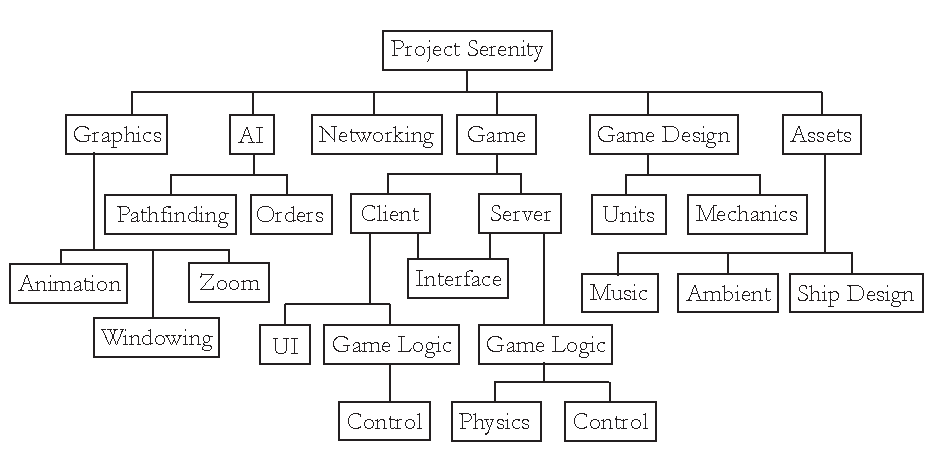
\includegraphics{res/wbs}
	\caption{Work Breakdown Structure of the game components.}
\end{figure*}

From the WBS we can further break the project down into components which are suited for weekly development cycles.

Term 2 releases will include a UI, an AI system and further improvements to the components as required. Assets such as music and additional ship designs are non-essential and will likely follow in a later release.

\begin{figure*}
	\label{dependency_tree}
	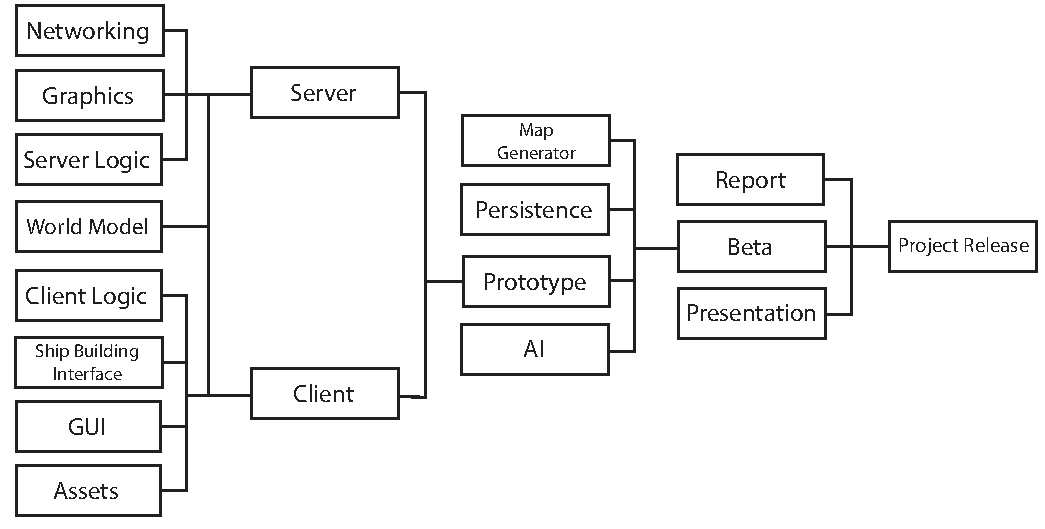
\includegraphics{res/dependency_tree}
	\caption[][-4.3em]{Component Dependency Graph.}
\end{figure*}

\begin{figure*}[h!]
	\label{gantt_chart}
	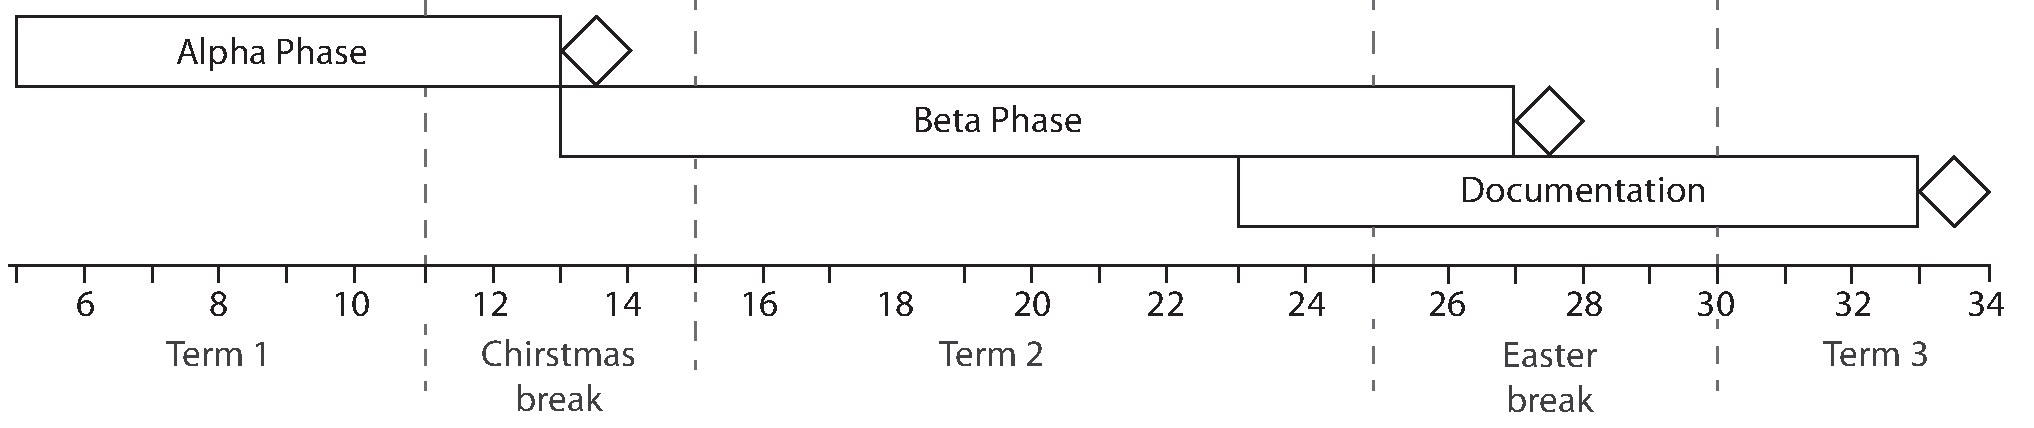
\includegraphics{res/gantt_chart_annotated}
	\caption{Phase level Gantt chart.}
\end{figure*}


\section{Schedule}

The project schedule has been mapped out in a stage-gate diagram (see figure \ref{stage_gate}) which breaks the project down into components, showing how tasks are allocated between team members. The Alpha phase has been carefully planned as it's the most relevant to the near future of the project and the team's work hours can only be definitely allocated in the near future. The Beta and Delivery phases have been planned in less (bust still sufficient) detail, allocating enough total time to address their components, however, the specific breakdown cannot be decided until the end of term 1, when the project progress is compared to the original schedule, the reaming time is reallocated as needed. Of course a stage-gate diagram has limitations in that overlapping phases cannot be represented easily, so we use a simple gantt chart (see figure \ref{gantt_chart}) to monitor phase transitions and ensure the project team is not mislead by a constrained representation of the schedule. 

The dependency tree shown in figure \ref{dependency_tree} reveals which components are directly dependant on others, and show how delays will propagate through the project. The project dependency diagram shows that potential loss is minimised after a prototype is complete, that is to say there are fewer critical dependancies from the prototype level onwards. This information emphasises the priority of the server and client components should the project schedule require revising at a later stage.





\begin{figure}
	\label{stage_gate}
	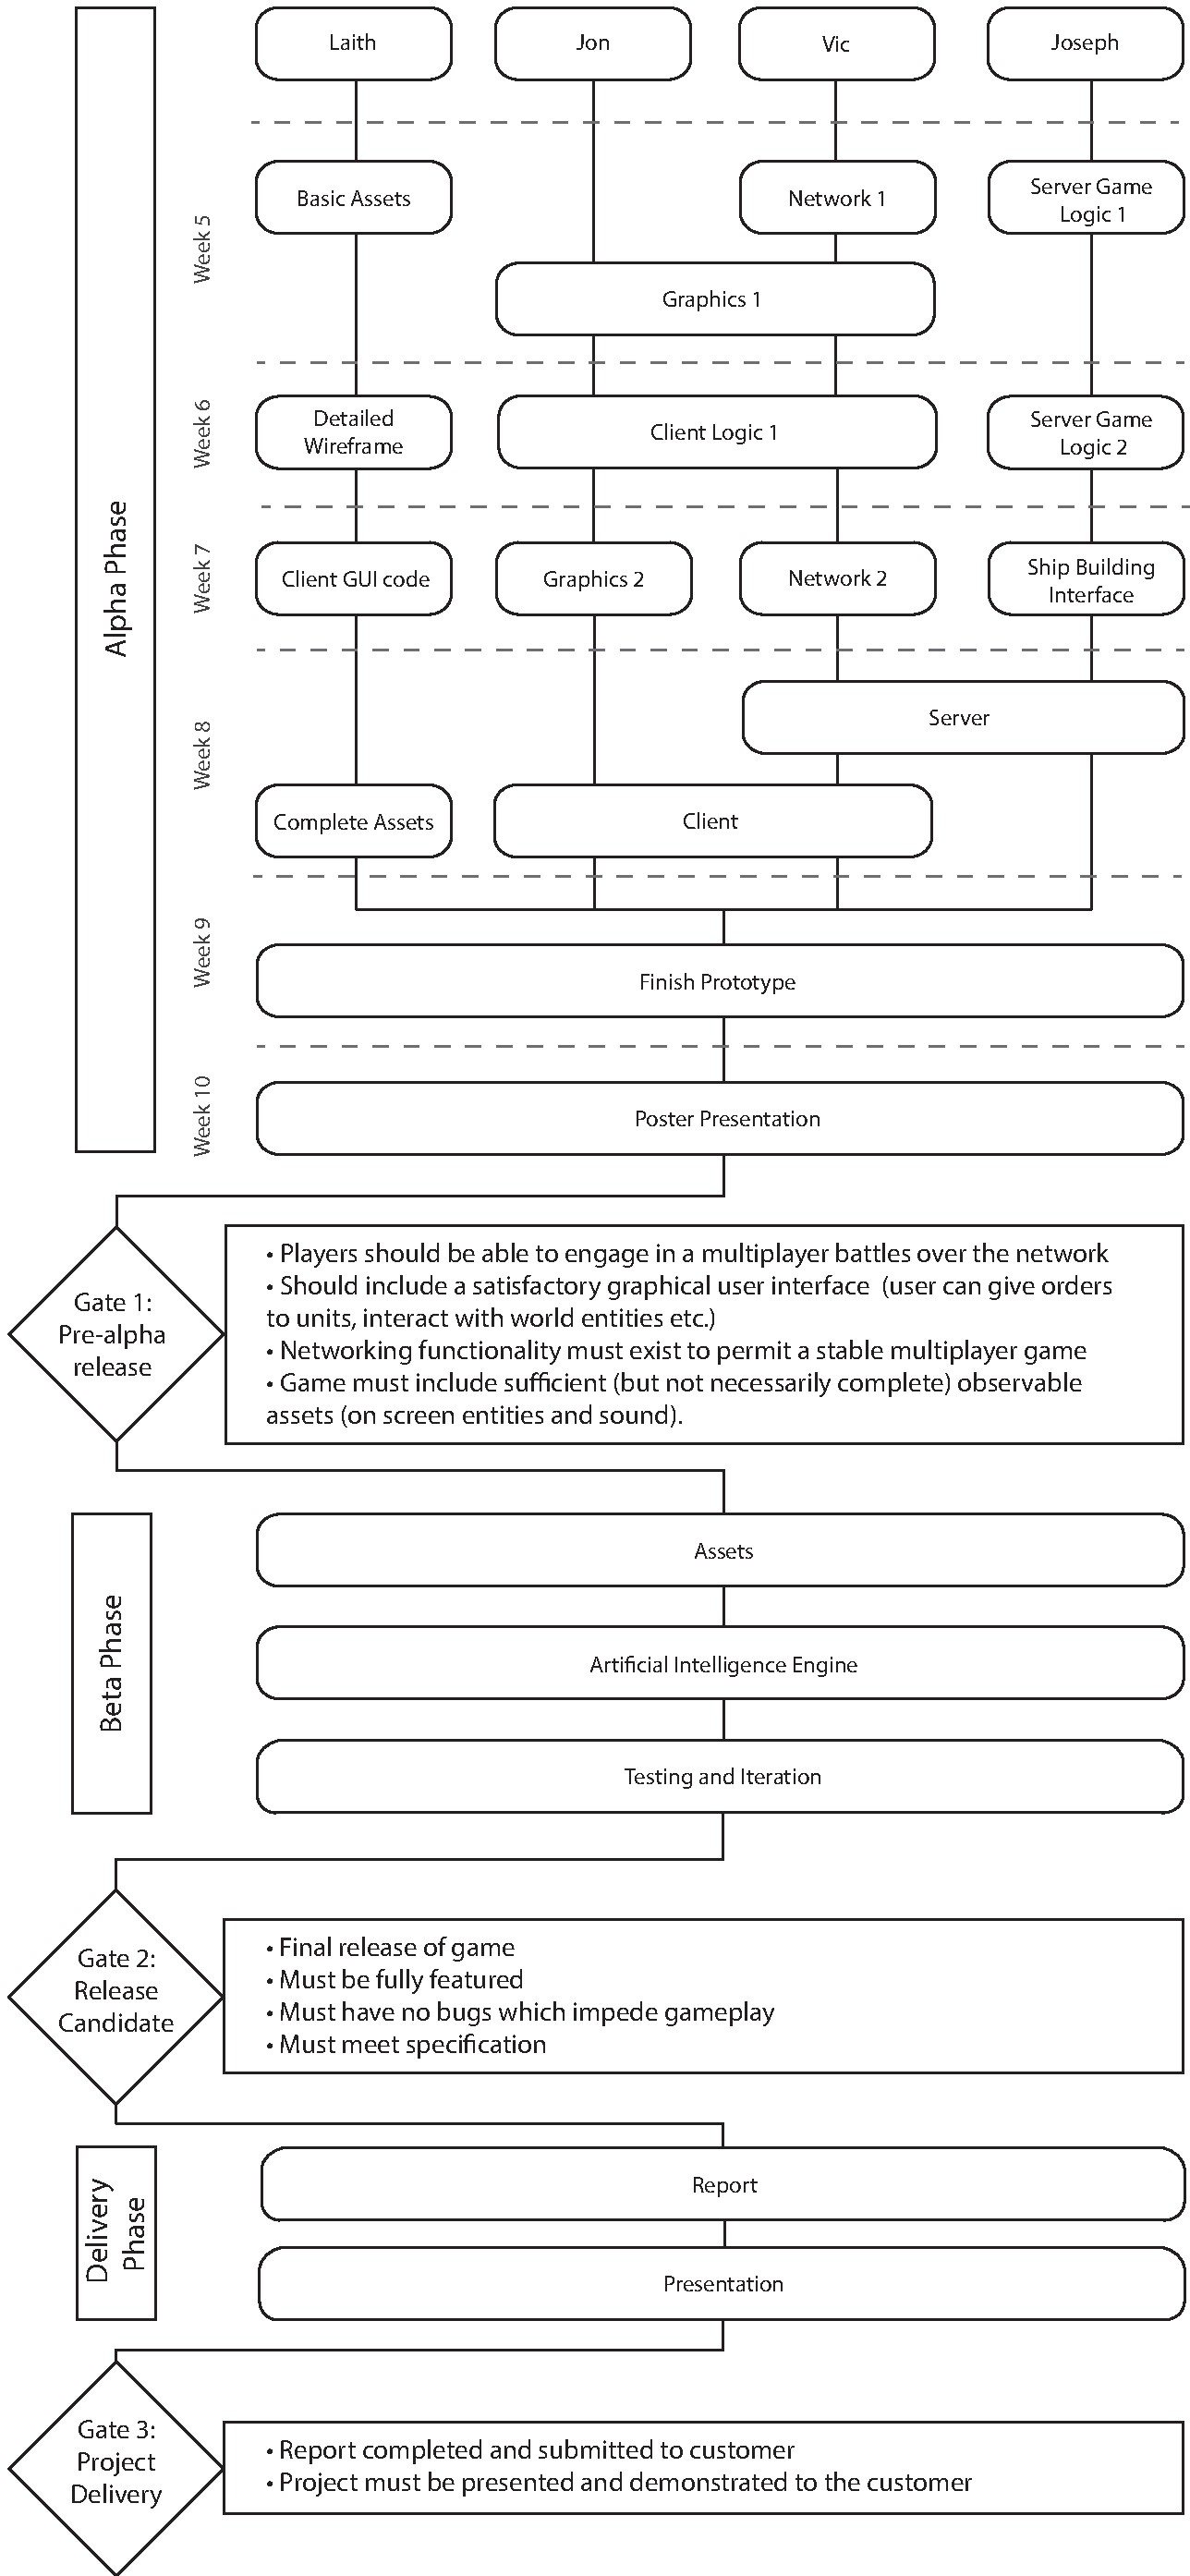
\includegraphics{res/stage_gate_diagram}
	\caption{Stage-gate model of work breakdown structure showing the division of labour across the various project phases. 
	The alpha phase is more thoroughly planned so we are able to see a weekly breakdown of tasks in the near future. The gates are project milestones, each of which details the requirements for proceeding through that gate into the next phase.}
\end{figure}
